\documentclass{beamer}
\usepackage[utf8]{inputenc}
\usepackage{graphicx}
\graphicspath{ {images/} }
\usepackage{utopia} %font utopia imported

\usetheme{Madrid}
\usecolortheme{default}
 
%Information to be included in the title page:
\title{Market value product summary using \\ Sentiment Analysis}
\author{Amritbani Sondhi\\Joy Shalom\\Sachin Shivashankara\\Akshay Manoharan}
\institute{Social Media Mining}
\date{Spring 2018}
 
 
 
\begin{document}
 
\frame{\titlepage}
 
\begin{frame}
\frametitle{Introduction}
\begin{itemize}
\item Perform Sentiment Analysis using data collected by twitter to perceive the summary between any two entities.
\item Rate their attributes 
\begin{itemize}
\item positive, negative and neutral
\item view the distribution of these attributes to comprehend them in a stronger way
\item geographic map, word cloud
\end{itemize}

\end{itemize}
\end{frame}

\begin{frame}
\frametitle{What we do?}
\begin{itemize}
\item Analyze the sentiments of tweets to compare two major multinational technology companies
\item Examples: Samsung and Apple
\end{itemize}
\end{frame}

\begin{frame}
\frametitle{Packages used}
\begin{itemize}
\item Tweepy: for accessing twitter data
\item Pandas: for using Panda dataframe
\item Numpy: for data manipulation
\item NLTK: for Sentiment Analysis
\item TextBlob: for Natural Language Processing
\item Bokeh: for Interactive Data Visualizations with bokeh server
\end{itemize}
\end{frame}

\begin{frame}
\frametitle{Sentiment Analysis}
\begin{itemize}
\item sometimes known as Opinion Mining or Emotion AI
\item refers to the use of natural language processing, text analysis, computational linguistics, and biometrics to systematically identify, extract, quantify, and study affective states and subjective information
\item \textit {Textblob} python package is used to perform sentiment analysis
\end{itemize}
\end{frame}

\begin{frame}
\frametitle{Sentiment Analysis}
{\Large Implementation}
\begin{itemize}
\item  \textit {Textblob} is used to classify the polarity of a tweet as positive, negative or neutral based on conceptualizing the entire text
\item  a number is assigned to each polarity of tweet.
\begin{itemize}
\item positive tweets are given ‘1’
\item negative tweets ‘-1’
\item neutral tweets ‘0’
\end{itemize}
\item associated each tweet to their polarity and added this information as a column in the data-frame
\item an \textit {attribute list}  is defined
\item  \textit {NLTK} package is used
\begin{itemize}
\item to tokenize every tweet
\item to compare if these tokens are in the attribute list
\end{itemize}
\item tweets that don’t have any of these attributes are then removed from the data frame
\end{itemize}
\end{frame}

\begin{frame}
\frametitle{Sentiment Analysis}
\begin{figure}
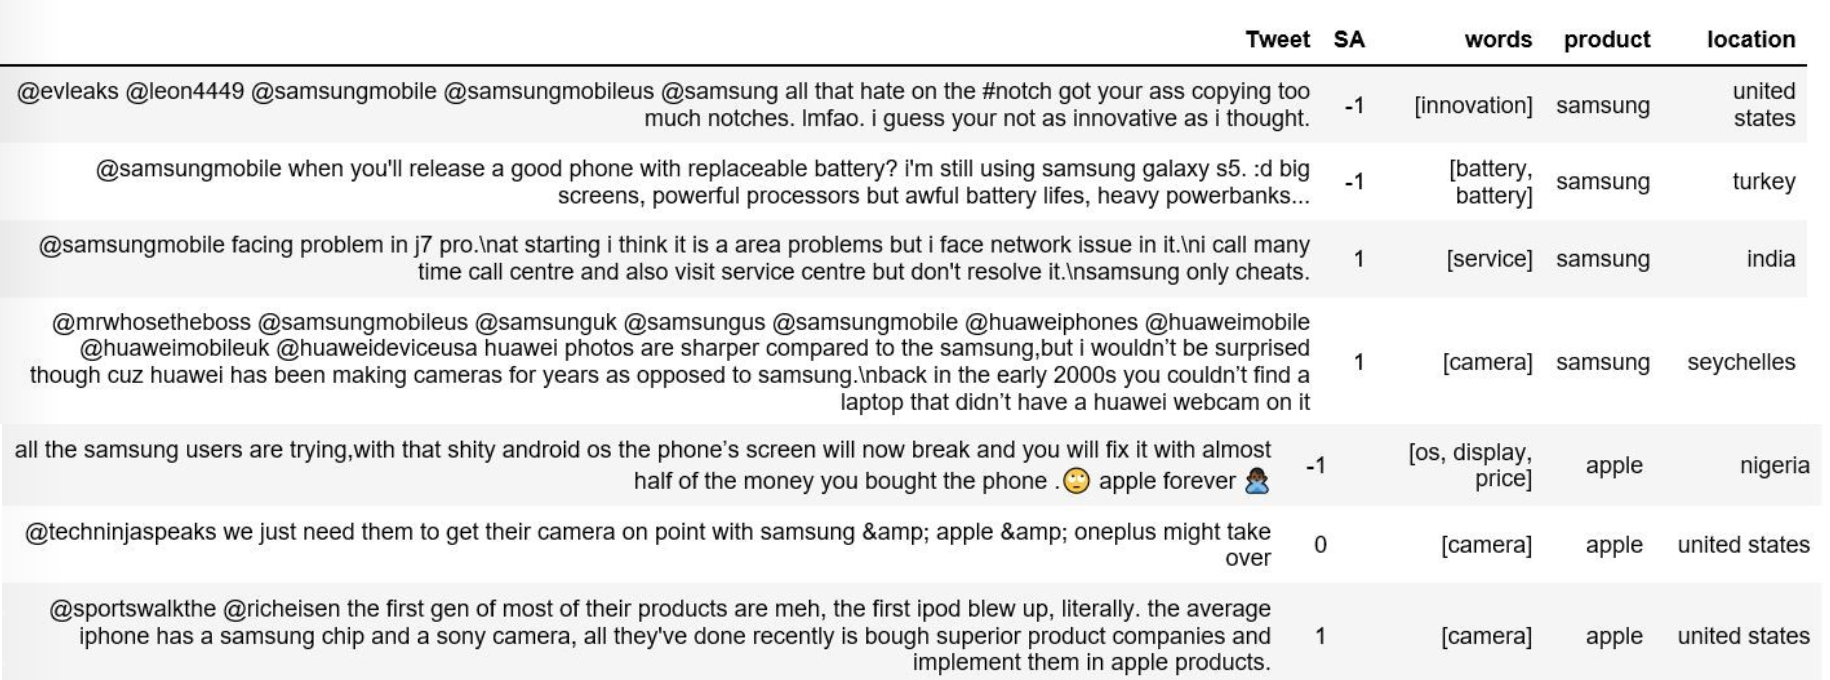
\includegraphics[scale=0.35]{sentiment}
\caption{ Dataframe retrieved from NLTK}
\end{figure}
\end{frame}

\begin{frame}
\frametitle{Sankey Diagram}
\begin{itemize}
\item   a visualization used to depict a flow from one set of values to another
\item best used  to represnt many-to-many mapping between two domains (e.g., samsung and apple)
\item used to associate words with their polarity
\item efficient way to reproduce the results of sentiment analysis
\end{itemize}
\end{frame}

\begin{frame}
\frametitle{Sankey Diagram}
{\Large Implementation}
\begin{itemize}
\item A complete list of all instances of positive words are available in a dictionary. 
\item  Set operation is performed in order to acquire only a unique set of positive words and pass it as an input to the sankey diagram. 
\item For linking them, source and target list has to be defined programmatically.
\item \textit{Plotly}
\begin{itemize}
\item Used for the implementation, where composing, editing and sharing the visualization is easier
\item It gives an interactive platform which shows data information while hovering
\end{itemize}
\end{itemize}
\end{frame}

\begin{frame}
\frametitle{Sankey Diagram}
\begin{figure}
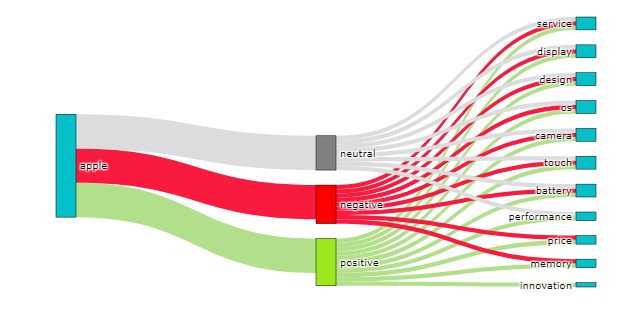
\includegraphics[scale=0.5]{aplsankey}
\caption{Sankey Diagram: Apple}
\end{figure}
\end{frame}

\begin{frame}
\frametitle{Sankey Diagram}
\begin{figure}
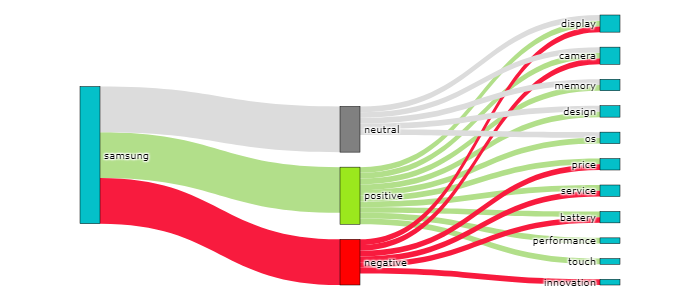
\includegraphics[scale=0.5]{samsankey}
\caption{Sankey Diagram: Samsung}
\end{figure}
\end{frame}


\begin{frame}
\frametitle{Word Cloud}
\begin{itemize}
\item Word cloud offers insight on which words are largely associated with a particular brand or entity
\item  The size of the word represents the frequency of its usage in tweets
\item The visualization from the word cloud is easy to interpret and shows how each attribute is compared to other attributes
\item It is convenient in associating a set of attributes to a brand
\end{itemize}
\end{frame}

\begin{frame}
\frametitle{Word Cloud}
{\Large Implementation}
\begin{itemize}
\item It is plotted for each sentiment polarity such as positive, negative and neutral for both Samsung and Apple
\item  A list of attributes for each polarity is given at its input
\item Based on the frequency of occurrence of these attributes the size of that attribute is decided by the word cloud, higher the frequency larger the size of the attribute
\end{itemize}
\end{frame}

\begin{frame}
\frametitle{Word Cloud}
{\large Positive Word Clouds}
\begin{figure}
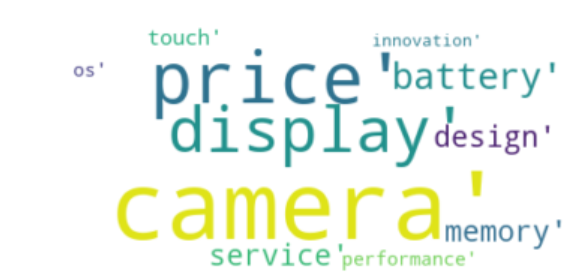
\includegraphics[scale=0.5]{sampos}
\caption{Positive Word Cloud: Samsung}
\end{figure}
\begin{figure}
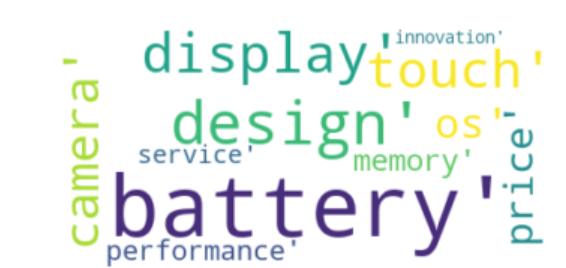
\includegraphics[scale=0.5]{aplpos}
\caption{Positive Word Cloud: Apple}
\end{figure}
\end{frame}

\begin{frame}
\frametitle{Word Cloud}
{\large Negative Word Clouds}
\begin{figure}
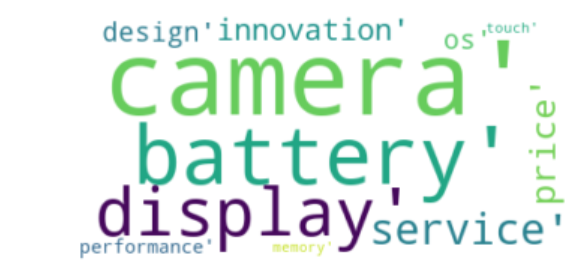
\includegraphics[scale=0.5]{samneg}
\caption{Sankey Diagram: Samsung}
\end{figure}
\begin{figure}
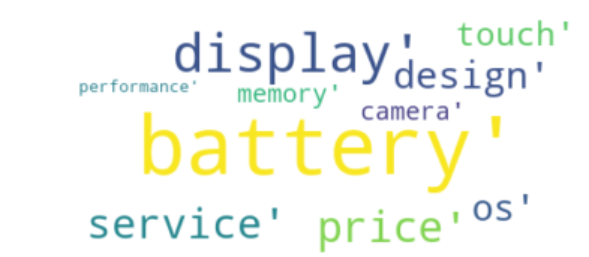
\includegraphics[scale=0.5]{aplneg}
\caption{Sankey Diagram: Apple}
\end{figure}
\end{frame}

\begin{frame}
\frametitle{Word Cloud}
{\large Neutral Word Clouds}
\begin{figure}
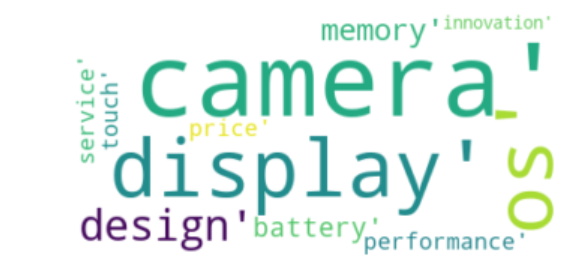
\includegraphics[scale=0.5]{samneu}
\caption{Neutral Word Cloud: Samsung}
\end{figure}
\begin{figure}
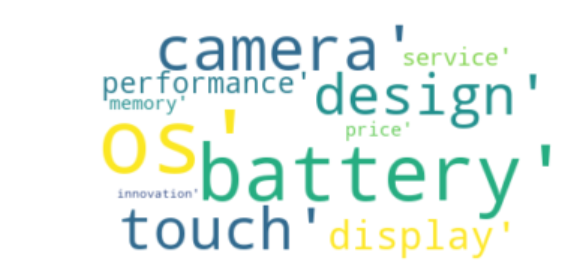
\includegraphics[scale=0.5]{aplneu}
\caption{Neutral Word Cloud: Apple}
\end{figure}
\end{frame}

\begin{frame}
\frametitle{Choropleth Map}
\begin{itemize}
\item Choropleth map is a thematic map in which areas are shaded or patterned in proportion to the measurement of the statistical variable being displayed on the map
\item It is used to see what nature of outlook a certain geographical area have on the entities compared
\item Tweets are grouped as positive, negative and neutral tweets and are associated with a location
\item The geographical areas are then given distinct colors based on the dominating sentiment polarity
\end{itemize}
\end{frame}

\begin{frame}
\frametitle{Choropleth Map}
{\Large Implementation}
\begin{itemize}
\item A .csv file which contains all states and its relevant state code is loaded 
\item Every country from the initial dataframe is compared with this list
\item  A new column is added where country code was present
\item For every country, the most dominant polarity is chosen based on the count of reviews over the region
\end{itemize}
\end{frame}

\begin{frame}
\frametitle{Choropleth Map}
\begin{figure}
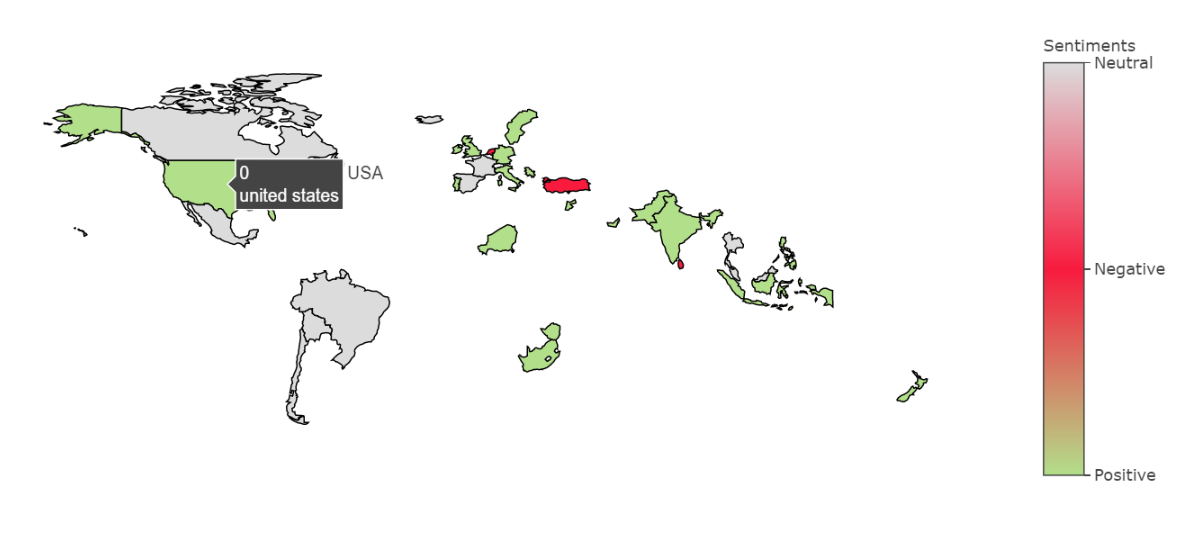
\includegraphics[scale=0.5]{samchoro}
\caption{Choropleth Map: Samsung}
\end{figure}
\end{frame}

\begin{frame}
\frametitle{Choropleth Map}
\begin{figure}
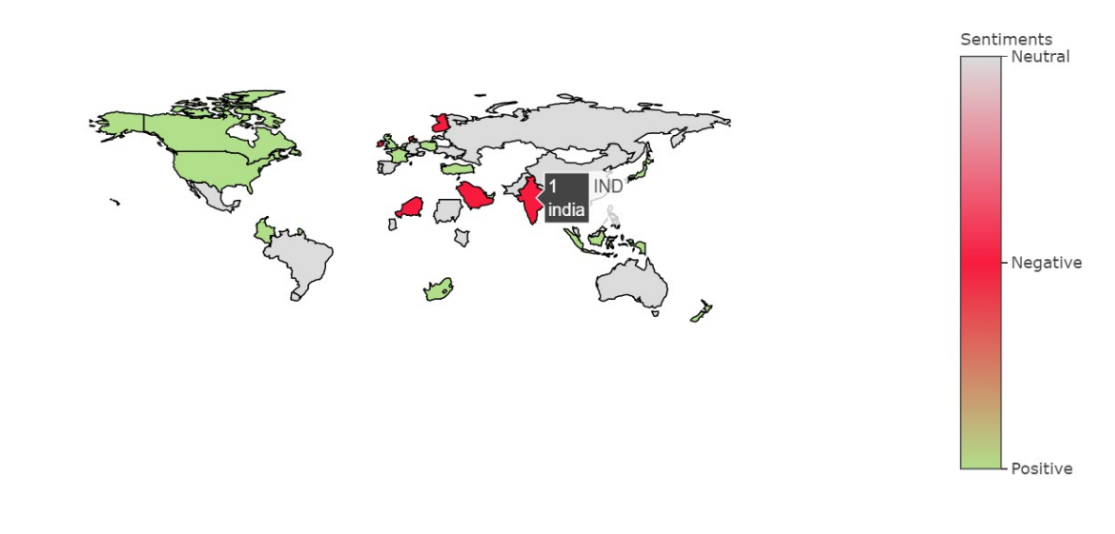
\includegraphics[scale=0.5]{aplchoro}
\caption{Choropleth Map: Apple}
\end{figure}
\end{frame}

\begin{frame}
\frametitle{User Interactions with the Server}
\begin{itemize}
\item \textit{Bokeh} is used to create the UI implementation of the project
\item It creates model objects in python and converts them into JSON format
\item The UI consists of the following widgets:
\begin{itemize}
\item TextHandler: to input the products to compare
\item Button: to generate analytical plots
\item Gridplot: for layouts
\end{itemize}
\item As \textit{plotly} and \textit{matplotlib} plots cannot be converted to bokeh figures and displayed, for better analysis on a button click event an image is plotted on the server and an interactive plot is launched on a new tab of the browser
\end{itemize}
\end{frame}

\begin{frame}
\frametitle{User Interactions with the Server}
\begin{figure}
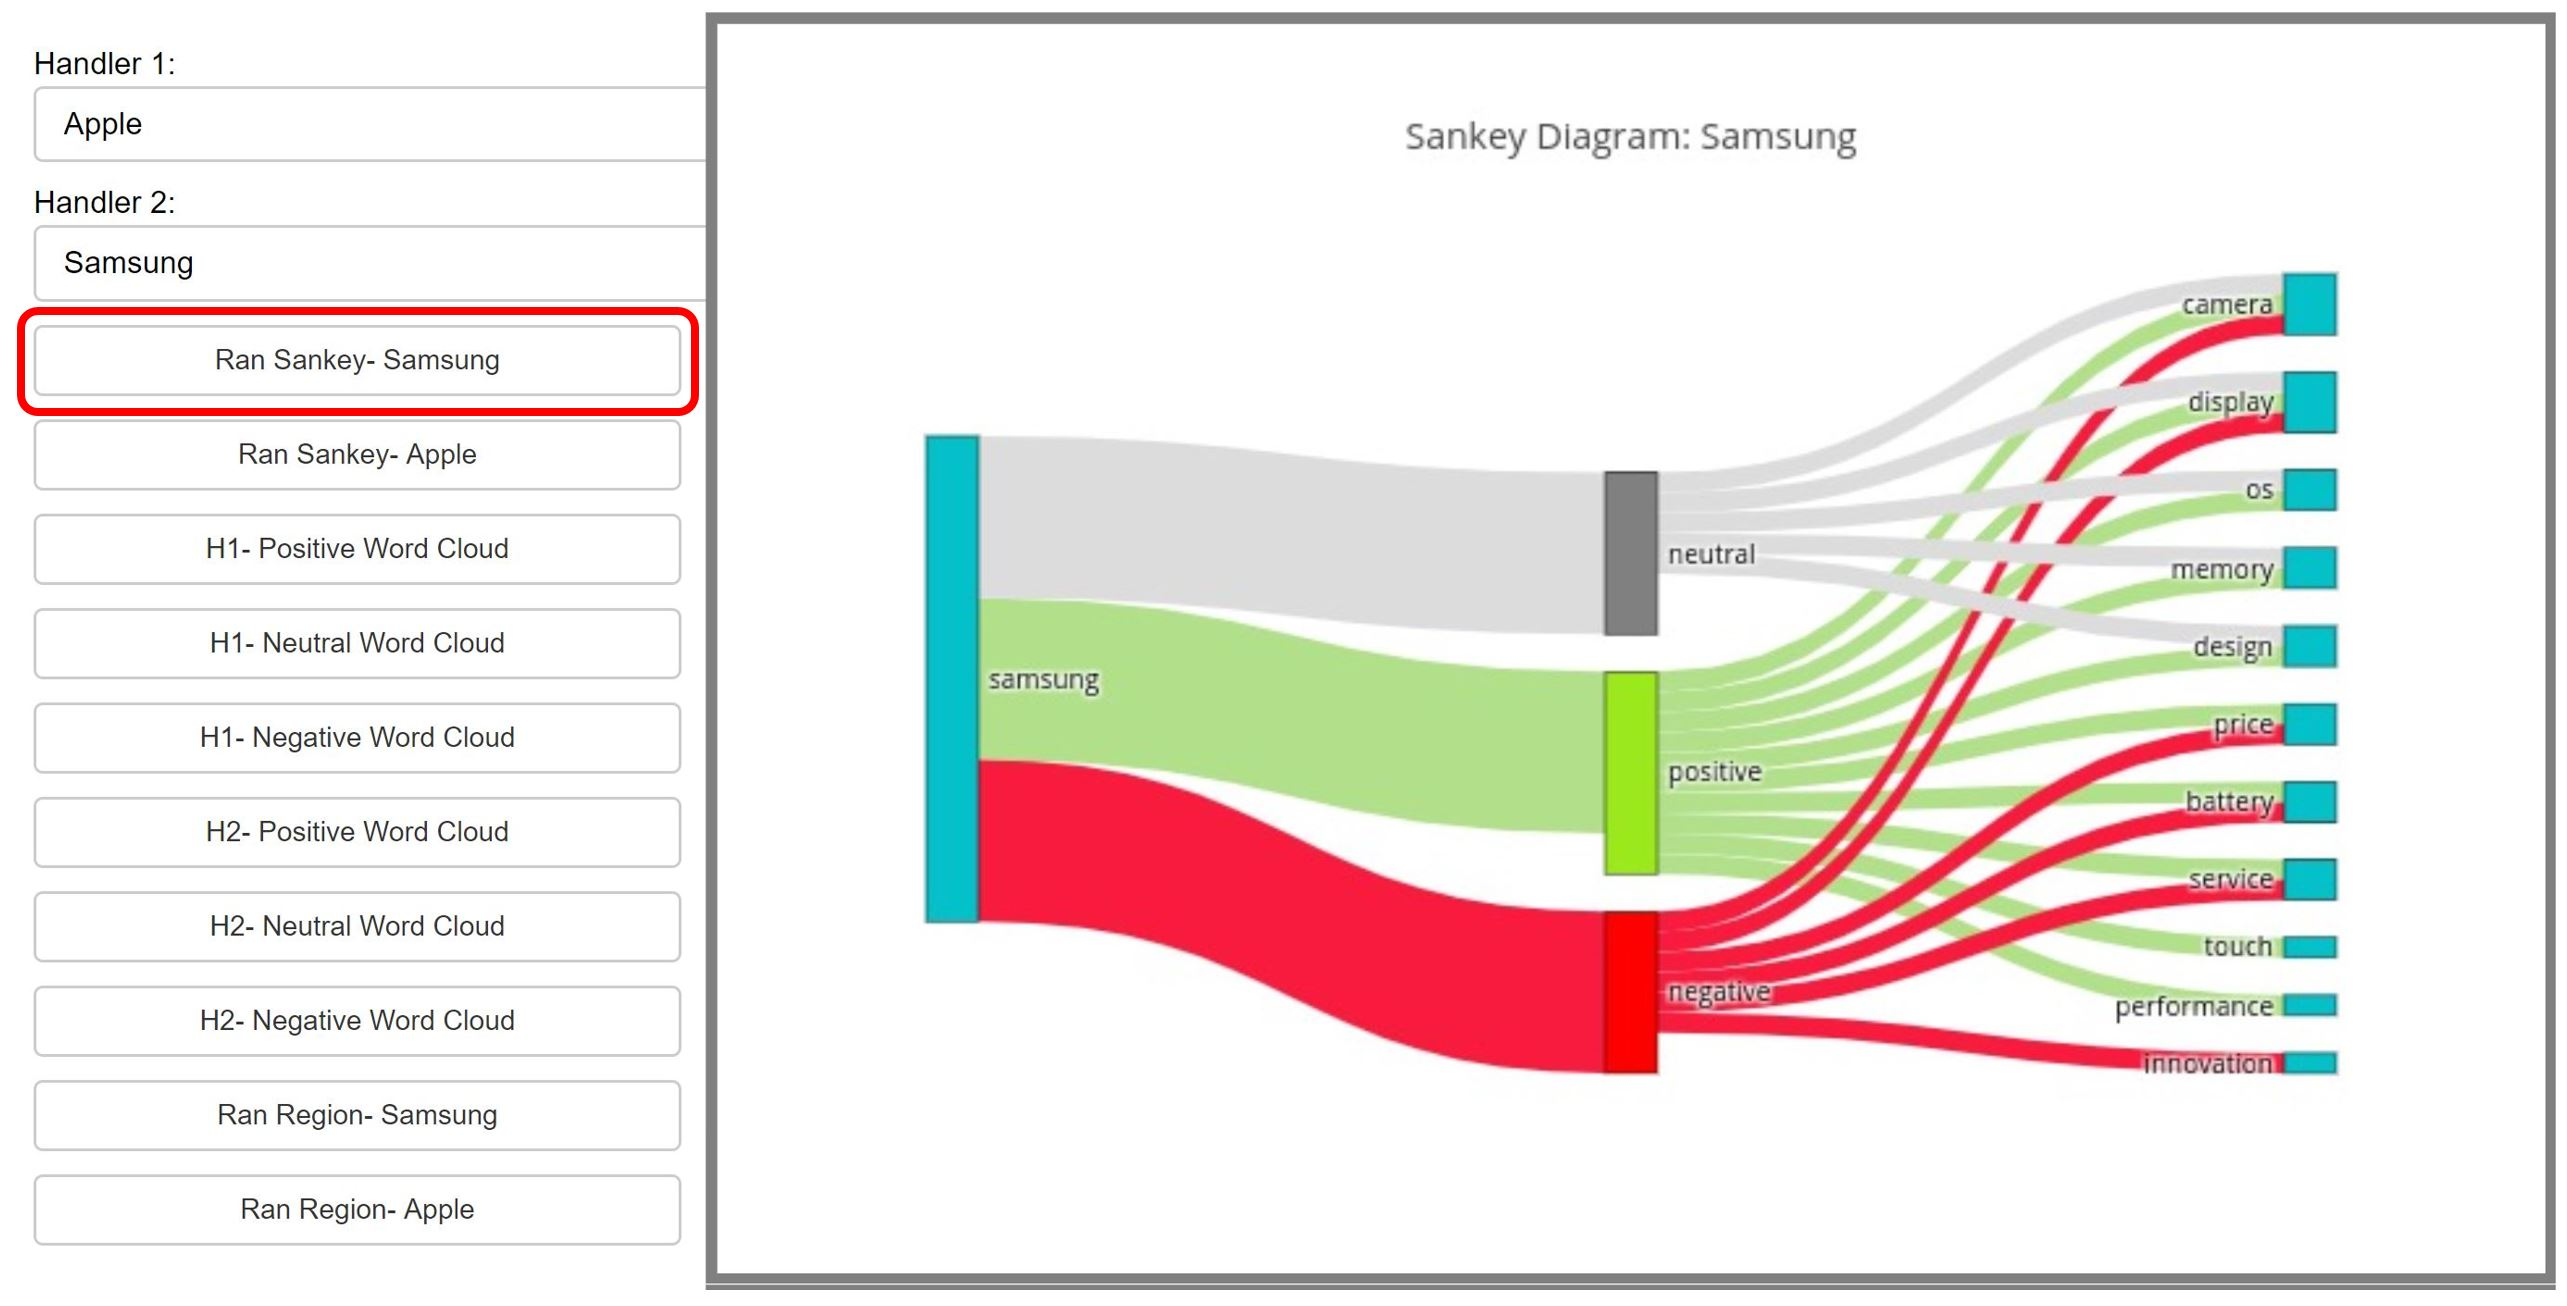
\includegraphics[scale=0.45]{Bokeh}
\caption{User Interface}
\end{figure}
\end{frame}

\begin{frame}
\frametitle{Observations}
{\Large Samsung}
\begin{itemize}
\item Positive outlook towards price, design and OS
\item Neutral outlook towards display 
\item Negative outlook towards battery and innovation
\item Choropleth map concludes that ‘Turkey, Netherlands and Sri Lanka’ has more negative outlook compared to other countries
\end{itemize}
\end{frame}

\begin{frame}
\frametitle{Observations}
{\Large Apple}
\begin{itemize}
\item Positive outlook towards design, camera and display
\item Neutral outlook towards battery
\item Negative outlook towards service
\item Choropleth map concludes that ‘Nigeria, Finland, Denmark, Ireland, Saudi Arabia and India’’ has more negative outlook compared to other countries
\end{itemize}
\end{frame}

%\begin{itemize}
%\item 
%\item
%\end{itemize}
 
\end{document}